%%%%%%%%%%%%%%%%%%%%%%%%%%%%%%%%%%%%%%%%%%%%%%%%%%%%%%%%%%%%%%%%%%%%%%%%%%%%%%%%
%	TRABAJO: Proyecto Integrador
%		Titulo: 	Desarrollo de IP cores con procesamiento de Redes de Petri 	
%					Temporales para sistemas multicore en FPGA					
%		Autores:	Juli�n Nonino												%					Carlos Renzo Pisetta										%		Director:	Orlando Micolini											
%%%%%%%%%%%%%%%%%%%%%%%%%%%%%%%%%%%%%%%%%%%%%%%%%%%%%%%%%%%%%%%%%%%%%%%%%%%%%%%%

% Path im�genes: ./marco_teorico/redes_de_petri/img
% Nombre predeterminado im�genes: petrixx
%	xx es el numero de imagen

\section{Redes de Petri con Arcos Inhibidores de peso unitario}
	\label{sec:arcos_inhibidores}

	En las Redes de Petri vistas anteriormente las transiciones est�n sensibilizadas cuando en las plazas de entrada existe una cantidad igual o mayor de tokens que el peso del arco que los une. Pero, en algunas situaciones, ser�a necesario que una transici�n se encuentre sensibilizada cuando no existan tokens en alguna de sus plazas de entrada. Para este fin existen los arcos inhibidores. Los arcos inhibidores se representan con una l�nea finalizada en un c�rculo. Se debe destacar que s�lo pueden ir desde plazas hacia las transiciones, nunca al rev�s. 

	\subsection{Definici�n matem�tica}

	Una Red de Petri marcada con arcos inhibidores queda definida por una 6-tupla de la siguiente manera:
	\begin{equation*}
		PN={P,T,I^-,I^+,H,m_0}
	\end{equation*}
	
	El elemento nuevo es la matriz \emph{H} llamada \textbf{matriz de inhibici�n} que es una matriz de $p$ filas y $t$ columnas. Siendo $p$ la cantidad de plazas de la red y $t$ la cantidad de transiciones.
	
	Es una matriz binaria, sus elementos solo pueden valer cero (0) o uno (1). Un \emph{uno} en la posici�n $a_{ij}$ indica que la plaza $i$ esta unida a la transici�n $j$ a trav�s de un arco inhibidor. 
	
	\subsection{Transiciones sensibilizadas en Redes de Petri con Arcos Inhibidores}
	
		Se pondr� como ejemplo la siguiente Red de Petri.
		\begin{figure}[H]
			\centering
			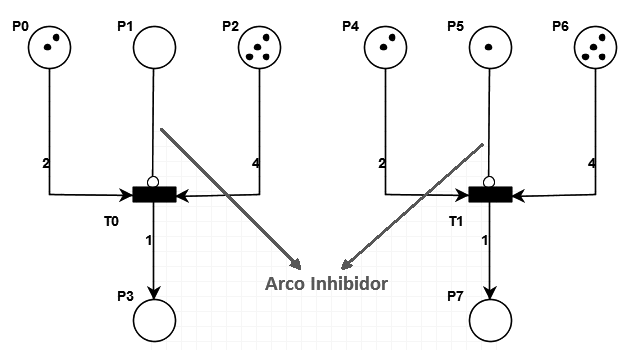
\includegraphics[width=.6\linewidth]{./marco_teorico/redes_de_petri/img/Petri15}
			\caption{ Ejemplo Red de Petri con Arco Inhibidor}
			\label{fig:Petri15}
		\end{figure}	
		
		En la Figura \ref{fig:Petri15}, se ve la representaci�n de un arco inhibidor y c�mo afecta a la transici�n. En la red de la izquierda, la transici�n $T0$ se encuentra sensibilizada mientras que en la red de la derecha la transici�n $T1$ no lo est�, por lo tanto no es posible que se dispare.
	
		Ahora, en una \textbf{\emph{Red de Petri con Arcos Inhibidores}}, se dice que una transici�n esta sensibilizada cuando se cumplen las siguientes condiciones:
		\begin{enumerate}
  			\item $\forall p_i \in I^-(t_j) : m(p_i) \geq W_{ij}$
  				\\
  				Siendo $W_{ij}$ el peso del arco (no inhibidor) que une la plaza $i$ con la transici�n $j$.
			\item Todas las plazas unidas a $t_j$ con arcos inhibidores no deben tener tokens.	
		\end{enumerate}
		
	\subsection{Ejecuci�n de una Red de Petri con Arcos Inhibidores}
			
		La ecuaci�n de estado para una Red de Petri con aros inhibidores toma la siguiente forma:
		\begin{equation}
			m_{i+1} = m_i  + I� \left[ \delta\;and\;f_H (m_i,\delta) \right]
			\label{eq:estado_petri_arcos_inhibidores}
		\end{equation}

		Como se ve, se agrega una funci�n $f$ que depende del marcado actual, del disparo a realizar y, de una funci�n $H$ que determina si una transici�n est� sensibilizada o no de acuerdo a  los arcos inhibidores. Esta funci�n toma solo valores ceros y unos, y al estar en una operaci�n $and$ con el disparo, puede inhibirlo y hacer que no produzca efectos.
		
		A continuaci�n se detalla la funci�n $f$.
		\begin{equation}
			f_H(m_i,\delta) = M_{=0}(m_i)\; nand \;(H � \delta)
			\label{eq:fun_inhibicion}
		\end{equation}
			
		La funci�n $M_{=0}()$ es una funci�n vectorial de $p$ elementos. Donde $p$ es la cantidad de plazas. Cada componente $k$ del resultado de la funci�n $M_{=0}()$ toma su valor de la siguiente ecuaci�n:
		\begin{equation}
			M_{=0}(m)_k =
				\begin{cases} 
					0 & \text{si } m_{ij} \neq 0
					\\
					1 & \text{si } m_{ij}= 0				
				\end{cases}		
			\label{eq:funcion_igual_cero}
		\end{equation}
